\documentclass[fleqn]{jbook}
\usepackage{physpub}

\begin{document}
\begin{question}{専攻 問題2}{}
電離層では空気分子は電子と陽イオンに電離されたプラズマ状態にある。電離層を伝搬する電磁波を考える。電離層は全体として中性であり電磁波に対して陽イオンは重いので動かず電子だけが動くとする。電子の質量は$m$、電荷を$-e$とし、また電子密度は$n$として常に一様であるとし、伝搬する電磁波によって生ずる磁場が電子の運動に及ぼす効果は無視できるものとする。平面波(周波数$\omega$、波数$k$)が電離層に垂直入射したとして以下の問いに答えよ。なおMaxwell方程式は
\begin{alignat}{2}
&\nabla \cdot \Vec{E} = 4\pi \rho &\hspace*{2cm} &\nabla \cdot \Vec{E} = \frac{\rho}{\varepsilon_0}\\
&\nabla \times \Vec{E} = -\frac{1}{c}\frac{\del \Vec{B}}{\del t} & &\nabla \times \Vec{E} = -\frac{\del \Vec{B}}{\del t}\eqname{2}\\
&\nabla \cdot \Vec{B} = 0 & &\nabla \cdot \Vec{B} = 0\\
&\nabla \times \Vec{B} = \frac{1}{c}\frac{\del \Vec{E}}{\del t} + \frac{4\pi}{c}\Vec{j} & &\nabla \times \Vec{B} = \mu_0\varepsilon_0\frac{\del \Vec{E}}{\del t} + \mu_0\Vec{j}\eqname{4}
\end{alignat}
と書かれる(左がC.G.S.系、右がM.K.S.系)。ここで$\Vec{E}$は電場、$\Vec{B}$は磁束密度、$\Vec{j}$は電流密度、$\varepsilon_0$は真空の誘電率、$\mu_0$は真空の透磁率をあらわす。必要ならば$\nabla\times(\nabla\times\Vec{A})=\nabla(\nabla\cdot\Vec{A})-\nabla^2\Vec{A}$の公式を用いてよい。またC.G.S.系、M.K.S.系のいずれの単位系を用いてもよい。

\begin{subquestions}
\SubQuestion
プラズマ中に誘起される電流密度$\Vec{j}$は、入射する電磁波の電場ベクトル$\Vec{E}$と電気伝導度$\sigma$を用い、$\Vec{j}=\sigma\Vec{E}$と書くことができる。まず外部磁場がゼロとして、電離層の電気伝導度$\sigma$を周波数$\omega$の関数として書け。

\SubQuestion
$k$と$\omega$の間の分散関係を求め電離層の屈折率($n\equiv ck/\omega$)を計算せよ。次に$\omega<\omega_p$のとき電磁波は伝搬できないことを示し、その物理的意味を説明せよ。ここで$\omega_p$はプラズマ周波数でありC.G.S.系では$\sqrt{4\pi ne^2/m}$、M.K.S.系では$\sqrt{ne^2/m\varepsilon_0}$で与えられる。

\end{subquestions}

次に電磁波の伝搬方向に一定磁場$\Vec{B}_0$がかかったとする。このとき磁場に対して右回りと左回りに円偏光した電磁波は異なる伝搬の仕方をする。$z$方向に伝搬する円偏光した電磁波の電場ベクトルは$\Vec{E}=E_0e^{i(kz-\omega t)}\frac{1}{\sqrt{2}}(\hat{\Vec{x}}\pm i\hat{\Vec{y}})$($\hat{\Vec{x}},\hat{\Vec{y}}$は各々$x$方向及び$y$方向の単位ベクトルで、+符号は右回り、−符号は左回り)と書けることを用い、以下に答えよ。


\begin{subquestions}[3]
\SubQuestion
右回り左回りそれぞれの電磁波に対する電離層の電気伝導度を$\omega,\omega_c$の関数として書け。ここで$\omega_c$はサイクロトロン周波数でありC.G.S.系では$eB_0/mc$、M.K.S.系では$eB_0/m$で与えられる。

\SubQuestion
右回り左回りそれぞれの電磁波に対する屈折率を$\omega,\omega_p$及び$\omega_c$の関数として求めよ。またこのとき一方の電磁波は$\omega<\omega_p$でも電離層を伝搬できることを示せ。

\end{subquestions}

\end{question}
\begin{answer}{専攻 問題2}{}
以下、M.K.S.系を利用する。
\begin{subanswers}
\SubAnswer
電流は$\Vec{j}=-en\dot{\Vec{x}}$であり、電場は一般に$\Vec{E}=\Vec{E}_0e^{i(\Vec{k}\cdot\Vec{x}-\omega t)}$と書ける。さて、
\begin{gather*}
\frac{\del \Vec{j}}{\del t} = -en\ddot{\Vec{x}}\\
m\ddot{\Vec{x}} = -e\Vec{E}
\end{gather*}
より、
\begin{equation}
\frac{\del \Vec{j}}{\del t} = \frac{ne^2}{m}\Vec{E} \eqname{dj/dt}
\end{equation}
となる。この式の左辺に、$\Vec{j}=\sigma\Vec{E}$の関係を代入して、
\[
\sigma\frac{\del \Vec{E}}{\del t} = \frac{ne^2}{m}\Vec{E}
\]
となる。最後にこの式に$\Vec{E}$の具体形を代入して、
\[
\sigma = i\frac{ne^2}{m\omega}
\]
を得る。


\SubAnswer
Maxwell方程式の\eqhref{4}式の両辺を$t$で微分すると、
\[
\nabla\times\frac{\del \Vec{B}}{\del t} = \mu_0\varepsilon_0\frac{\del^2 \Vec{E}}{\del t^2} + \mu_0\frac{\del \Vec{j}}{\del t}
\]
となる。この式の左辺にMaxwell方程式の\eqhref{2}と、問1で得た\eqhref{dj/dt}式を代入すると、
\begin{align}
\nabla^2 \Vec{E} &= \mu_0\varepsilon_0\frac{\del^2 \Vec{E}}{\del t^2} + \mu_0\frac{\del \Vec{j}}{\del t} \eqname{lap_e}\\
&= \mu_0\varepsilon_0\frac{\del^2 \Vec{E}}{\del t^2} + \mu_0\frac{ne^2}{m}\Vec{E} \nonumber
\end{align}
を得る。この式に$\Vec{E}$の具体形を代入すると、
\begin{align*}
-k^2 &= -\mu_0\varepsilon_0\omega^2 + \mu_0\frac{ne^2}{m}\\
&= -\frac{\omega^2}{c^2}\left(1-\left(\frac{\omega_p}{\omega}\right)^2 \right) \qquad (\omega_p\text{はプラズマ周波数})
\end{align*}
となり、従って、
\[
n \equiv \frac{ck}{\omega} = \sqrt{1-\left(\frac{\omega_p}{\omega}\right)^2}
\]
を得る。

さて、$\omega<\omega_p$の時は屈折率は虚数となるため、電場が電離層に入射しても、電場は指数関数的に減少する。よって、電場は電離層を伝搬できずに、全反射される。


\SubAnswer
電子の運動方程式は、
\[
m\dot{\Vec{v}} = -e\Vec{E} - e\Vec{v}\times\Vec{B}_0
\]
である。さて、
\begin{align}
\Vec{E} &= \frac{E_0}{\sqrt{2}}(\hat{\Vec{x}} \pm i\hat{\Vec{y}})e^{i(kz-\omega t)}\eqname{e}\\
\Vec{v} &= \frac{v_0}{\sqrt{2}}(\hat{\Vec{x}} \pm i\hat{\Vec{y}})e^{i(kz-\omega t)}\\
\Vec{B}_0 &= B_0\hat{\Vec{z}}
\end{align}
と置くと、
\begin{align}
\Vec{v}\times\Vec{B}_0 &= \frac{v_0 B_0}{\sqrt{2}}(\hat{\Vec{x}} \pm i\hat{\Vec{y}})\times \hat{\Vec{z}}e^{i(kz-\omega t)}\nonumber\\
&=\pm i\frac{v_0 B_0}{\sqrt{2}}(\hat{\Vec{x}} \pm i\hat{\Vec{y}}) e^{i(kz-\omega t)}\eqname{vb}
\end{align}
となる。よって、電子の運動方程式に\eqhref{e},\eqhref{vb}式を代入して、
\[
v_0(-im\omega \pm ieB_0) = -eE_0
\]
より、
\begin{equation}
v_0 = \frac{-ieE_0}{m(\omega \mp \omega_c)} \qquad (\omega_c \text{はサイクロトロン周波数})
\end{equation}
を得る。電流密度の大きさは、$j_0=-env_0$と書けるので、
\[
j_0 = -env_0 = \frac{ine^2}{m(\omega \mp \omega_c)}E_0
\]
より、電気伝導度は、
\begin{equation}
\sigma = \frac{ine^2}{m(\omega \mp \omega_c)} \eqname{sig}
\end{equation}
となる。


\SubAnswer
問2で得た\eqhref{lap_e}式を利用して、
\begin{align*}
&\nabla^2 \Vec{E} = \mu_0\varepsilon_0\frac{\del^2 \Vec{E}}{\del t^2} + \mu_0\frac{\del \Vec{j}}{\del t}\\
&\Longleftrightarrow k^2 \Vec{E} = \mu_0(\varepsilon_0\omega^2 + i\omega\sigma)\Vec{E}
\end{align*}
となる。この式を屈折率の定義の形に変形すると、
\begin{align*}
&\left(\frac{kc}{\omega}\right)^2 = 1+\frac{i}{\varepsilon_0\omega}\sigma \qquad (\leftarrow \eqhref{sig}\text{式を代入})\\
&\Longleftrightarrow n_{\pm}^2 =1-\frac{ne^2}{\varepsilon_0 m\omega(\omega\mp\omega_c)}\\
&\Longleftrightarrow n_{\pm}^2 =1-\frac{\omega_p^2}{\omega(\omega\mp\omega_c)}
\end{align*}
となるので、屈折率は、
\[
n_{\pm} = \sqrt{1-\frac{\omega_p^2}{\omega(\omega\mp\omega_c)}}
\]
となる。

さて、$x\equiv \omega/\omega_p,\ \omega'\equiv \omega_c/\omega_p$とおくと、
\[
n_{\pm}(x) = \sqrt{1-\frac{1}{x(x\mp\omega')}}
\]
となる。また、$f_{\pm}(x)\equiv n_{\pm}^2(x)$とすると、$f_{\pm}(x)\ge 0$となる周波数領域では電磁波が伝搬できることになる。次に$f_{\pm}(x)$のグラフを示す。(ただし、$\omega'<1$の場合)
\begin{center}
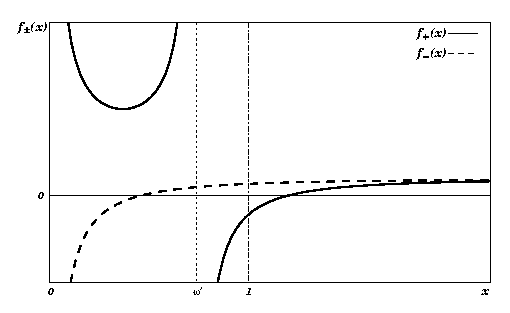
\includegraphics[clip]{1999phy2-1.eps}
\end{center}
このグラフから分かるように、$x<1$つまり$\omega<\omega_p$の領域でも$f_+(x)>0$となる領域があるため、この時$n_+(x)$は実数となる。従って、右回りの電磁波は$\omega<\omega_p$でも伝搬できる。

\end{subanswers}
\end{answer}



\end{document}
